\documentclass[final,3p,authoryear]{elsarticle}

\usepackage{lipsum}
 \usepackage{graphics}
\usepackage[]{algorithm2e}
 \usepackage{setspace}
%% or use the graphicx package for more complicated commands
 \usepackage{graphicx}
%% or use the epsfig package if you prefer to use the old commands
 \usepackage{epsfig}
 \usepackage{subfigure}

%% The amssymb package provides various useful mathematical symbols
\usepackage{amssymb}
%% The amsthm package provides extended theorem environments
 \usepackage{amsthm,amsmath}
 \usepackage{multirow}
 \usepackage{setspace}
 \usepackage{CJK}
 \usepackage{float}
 \usepackage{pdfpages}
 \usepackage{mathtools}
% \usepackage{natbib}
 \restylefloat{table}
 \onehalfspacing



\makeatletter
\def\ps@pprintTitle{%
	\let\@oddhead\@empty
	\let\@evenhead\@empty
	\def\@oddfoot{}%
	\let\@evenfoot\@oddfoot}
\makeatother

\usepackage{etoolbox}
\patchcmd{\abstract}{Abstract}{}{}{}

\begin{document}

\begin{frontmatter}

\title{MATH 6740: Financial Mathematics and Simulation\\
	Homework 3 solutions/presentation}

\author[rvt]{Jubiao ``Jack'' Yang}

\address[rvt]{Rensselaer Polytechnic Institute, Troy, NY 12180}

\begin{abstract}
	Solve Exercise Problems 1.4, 1.6, and 1.7 in \cite[Chapter 1, p.~42-43]{shreve2004stochastic}.
\end{abstract}


\end{frontmatter}

\section{Exercise 1.4}
	\subsection{Exercise 1.4 i)}
		First follow \cite[Example 1.2.5, p.~11-12]{shreve2004stochastic} to construct a uniformly distributed random variable $X$ taking values in $\left[0,1\right]$ and defined on infinite coin-toss space $\Omega_\infty$ where $p_H=p_T=0$, by defining
		\begin{equation}
			Y_n(\omega|_n)=
			\begin{cases}
				1\qquad \mathrm{if~} \omega|_n=H,\\
				0\qquad \mathrm{if~} \omega|_n=T,
			\end{cases}
		\end{equation}
		which is an indicator of whether the result of the $n^\mathrm{th}$ toss is $\omega|_n=H$, where $\omega \in \Omega_\infty$, and
		\begin{equation}
			X=\sum\limits_{n=1}^{\infty} \frac{Y_n}{2^n}
			.
		\end{equation}
		\cite[Example 1.2.5, p.~11-12]{shreve2004stochastic} concluded that $X\sim U(0,1)$.
		Next \cite[Example 1.2.6, p.~12-13]{shreve2004stochastic} showed that with the probability density function and cumulative distribution function of the standard normal distribution being:
		\begin{equation}
			\varphi(x)=\frac{1}{2\pi} e^{-\frac{x^2}{2}}
			,
		\end{equation}
		\begin{equation}
			N(x)=\int_{-\infty}^{x} \varphi(\xi) d\xi
			,
		\end{equation}
		we can defined a new random variable $Z=N^{-1}(X)$, where $N^{-1}(\cdot)$ is the inverse function of $N(\cdot)$, which exists because $N(\cdot)$ is strictly increasing. For $\forall -\infty < a \leq b < \infty$, we have
		\begin{eqnarray}
			\mu_Z[a,b]&=&P(\omega \in \Omega_\infty| a \leq Z(\omega) \leq b)
			\nonumber\\
			&=&P(\omega \in \Omega_\infty| a \leq N^{-1}(X(\omega)) \leq b)
			\nonumber\\
			&=&P(\omega \in \Omega_\infty| N(a) \leq X(\omega) \leq N(b))
			\nonumber\\
			&=&N(b)-N(a)=\int_{a}^{b} \varphi(\xi) d\xi
			.
		\end{eqnarray}
		Therefore
		\begin{equation}
			Z=N^{-1}(X)=N^{-1}(\sum\limits_{n=1}^{\infty} \frac{Y_n}{2^n}) \sim N(0,1)
			.
		\end{equation}
		
	\subsection{Exercise 1.4 ii)}
		Define the indicator function $Y_n(\omega|_n)$ as before:
		\begin{equation}
			Y_n(\omega|_n)=
			\begin{cases}
				1\qquad \mathrm{if~} \omega|_n=H,\\
				0\qquad \mathrm{if~} \omega|_n=T,
			\end{cases}
		\end{equation}
		and a sequence of random variables $\{X_n\}_{n=1}^{\infty}$ on $\Omega_\infty$, where each element only depends on the results of the first $n^\mathrm{th}$ tosses, as:
		\begin{equation}
			X_n=\sum\limits_{i=1}^{n} \frac{Y_i}{2^i}
			.
		\end{equation}
		The binary number $\overline{Y_1 Y_2 \cdots Y_n}=\sum\limits_{i=1}^{n} 2^{n-i} Y_i$ is a random variable taking all integer values between $0$ and $2^n-1$ with equal probability $1/2^n$, therefore $X_n=\frac{1}{n} \overline{Y_1 Y_2 \cdots Y_n}$ is a random variable, with equal probability $1/2^n$, taking values in the set $\{0, \frac{1}{2^n}, \cdots, \frac{2^n-1}{2^n}\}$, which is an arithmetic series from $0$ to $(2^n-1)/2^n$ with common distance $1/2^n$, therefore:
		\begin{equation}
			P(\omega \in \Omega| \frac{k-1}{2^n} \leq X_n < \frac{k}{2^n}, k \in \mathbb{Z},k \in [1,2^n]) = \frac{1}{2^n}
			.
		\end{equation}
		Now define a sequence of random variables $\{Z_n\}_{n=1}^{\infty}$, with each element $Z_n = N^{-1}(X_n)$, then for $\forall -\infty < a \leq b < \infty$, there is:
		\begin{eqnarray}
			\mu_{Z_n}[a,b]&=&P(\omega \in \Omega_\infty| a \leq Z_n(\omega) \leq b)
			\nonumber\\
			&=&P(\omega \in \Omega_\infty| a \leq N^{-1}(X_n(\omega)) \leq b)
			\nonumber\\
			&=&P(\omega \in \Omega_\infty| N(a) \leq X_n(\omega) \leq N(b))
			\nonumber\\
			&=&P(\omega \in \Omega_\infty| \frac{\lceil N(a)\cdot 2^n \rceil}{2^n} \leq X_n(\omega) < \frac{\lfloor N(b)\cdot 2^n \rfloor + 1}{2^n})
			\nonumber\\
			&=& \frac{\lfloor N(b)\cdot 2^n \rfloor - \lceil N(a)\cdot 2^n \rceil + 1}{2^n}
			\nonumber\\
			&=&N(b)-N(a) + \frac{O(1)}{2^n}
			,
		\end{eqnarray}
		therefore
		\begin{equation}
			\lim\limits_{n \to \infty} \mu_{Z_n}[a,b] = \mu_Z[a,b]
			,
		\end{equation}
		and
		\begin{equation}
			\lim\limits_{n \to \infty} Z_n(\omega) = Z(\omega),\quad \forall \omega \in \Omega_\infty
			,
		\end{equation}
		where $Z_n(\omega)$ is defined, with the inverse of the standard normal distribution $N^{-1}(\cdot)$, as:
		\begin{equation}
			Z_n=N^{-1}(X_n)=N^{-1}(\sum\limits_{i=1}^{n} \frac{Y_i}{2^i})
			.
		\end{equation}
		
\section{Exercise 1.6}
	\subsection{Exercise 1.6 i)}
		\begin{eqnarray}
			E[e^{uX}] &=& \int_{-\infty}^{\infty} e^{ux} f(x) dx
			\nonumber\\
			&=& \int_{-\infty}^{\infty} e^{ux} \frac{1}{\sigma \sqrt{2\pi}} e^{-\frac{(x-\mu)^2}{2\sigma^2}} dx
			\nonumber\\
			&=& \int_{-\infty}^{\infty} \frac{1}{\sigma \sqrt{2\pi}} e^{-\frac{x^2 - (2\mu + 2u \sigma^2)x + \mu^2}{2\sigma^2}} dx
			\nonumber\\
			&=& \int_{-\infty}^{\infty} \frac{1}{\sigma \sqrt{2\pi}} e^{-\frac{[x-(\mu + u\sigma^2)]^2 - 2\mu u \sigma^2 - u^2 \sigma^4}{2\sigma^2}} dx
			\nonumber\\
			&=& e^{u \mu + \frac{1}{2}u^2 \sigma^2} \int_{-\infty}^{\infty} \frac{1}{\sigma \sqrt{2\pi}} e^{-\frac{[x-(\mu + u\sigma^2)]^2}{2\sigma^2}} dx
			\nonumber\\
			&=& e^{u \mu + \frac{1}{2}u^2 \sigma^2}
			.
		\end{eqnarray}
	
	\subsection{Exercise 1.6 ii)}
		For the convex function $\varphi(x)=e^{ux}$:
		\begin{equation}
			E[\varphi(X)] = E[e^{uX}] = e^{u \mu + \frac{1}{2}u^2 \sigma^2} \geq e^{u\mu} = \varphi(E[X])
			,
		\end{equation}
		which satisfies Jensen's inequality.
		
\section{Exercise 1.7}
	\subsection{Exercise 1.7 i)}
		\begin{eqnarray}
			f(x) &=& \lim\limits_{n \to \infty} f_n(x) = \lim\limits_{n \to \infty} \frac{1}{\sqrt{2n\pi}} e^{-\frac{x^2}{2n}}
			\nonumber\\
			&=& \lim\limits_{n \to \infty} \frac{1}{\sqrt{2n\pi}} \sum\limits_{i=0}^{\infty} \frac{1}{i!} \left( -\frac{x^2}{2n} \right)^i
			\nonumber\\
			&=& \frac{1}{\sqrt{2\pi}} \lim\limits_{n \to \infty} \left( \frac{1}{n^{1/2}} - \frac{x^2}{2n^{3/2}} + \frac{x^4}{8n^{5/2}} + f(x)O(\frac{1}{n^{7/2}}) \right)
			\nonumber\\
			&=& 0
			.
		\end{eqnarray}
		
	\subsection{Exercise 1.7 ii)}
		Since $f_n(x)=\frac{1}{\sqrt{2n\pi}} e^{-\frac{x^2}{2n}}$ is essentially the probability density function of a random variable with normal distribution $X \sim N(0,n)$, therefore $\int_{-\infty}^{\infty} f_n(x) dx = 1$, thus
		\begin{equation}
			\lim\limits_{n \to \infty} \int_{-\infty}^{\infty} f_n(x) dx = 1
			.
		\end{equation}
		
	\subsection{Exercise 1.7 iii)}
		The Monotone Convergence Theorem requires that
		\begin{equation}
			0 \leq f_1 \leq f_2 \leq \cdots \quad \mathrm{almost~everywhere}
			.
		\end{equation}
		In this instance, the range of $x$ where $f_n(x)>f_{n+1}(x)$ can be determined with, since $f_n(x)>0$:
		\begin{eqnarray}
			\frac{f_n(x)}{f_{n+1}(x)} = \frac{\sqrt{n+1} \cdot e^{-\frac{x^2}{2n}}}{\sqrt{n} \cdot e^{-\frac{x^2}{2(n+1)}}} > 1
			\quad\Rightarrow\quad
			e^{\frac{x^2}{2n}-\frac{x^2}{2(n+1)}} &<& \sqrt{\frac{n + 1}{n}}
			\nonumber\\
			e^{\frac{x^2}{2n(n+1)}} &<& \sqrt{\frac{n + 1}{n}}
			\nonumber\\
			\frac{x^2}{2n(n+1)} &<& \frac{1}{2} \ln{\frac{n + 1}{n}}
			\nonumber\\
			-n(n+1)\ln{\frac{n + 1}{n}} < &x& < n(n+1)\ln{\frac{n + 1}{n}}
			,
		\end{eqnarray}
		which is a non-trivial range. Therefore the fact that
		\begin{equation*}
			\lim\limits_{n \to \infty} \int_{-\infty}^{\infty} f_n(x) dx \neq \int_{-\infty}^{\infty} f(x) dx
		\end{equation*}
		does not violate the Monotone Convergence Theorem.
	

	
\appendix

\section{Original Homework Questions (attached)}
%	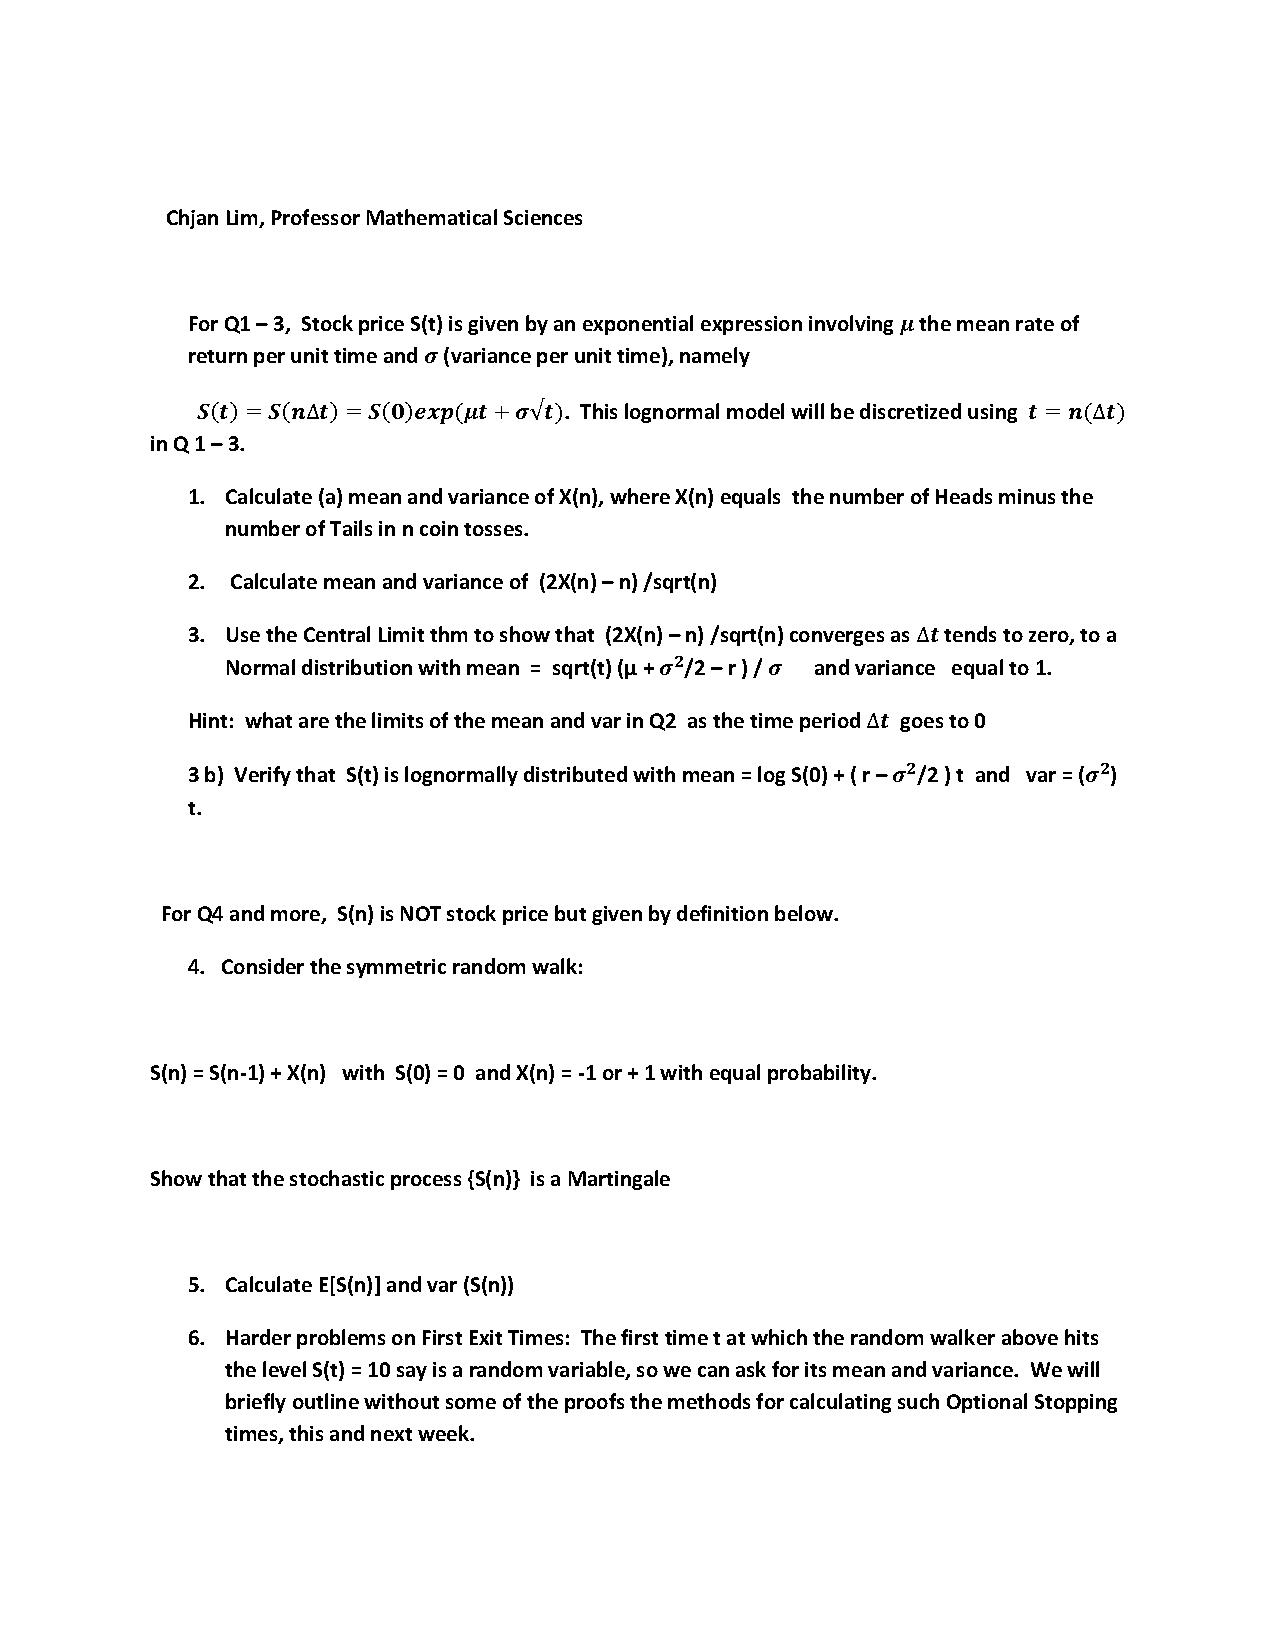
\includepdf[pages={1}]{worksheet216.pdf}
	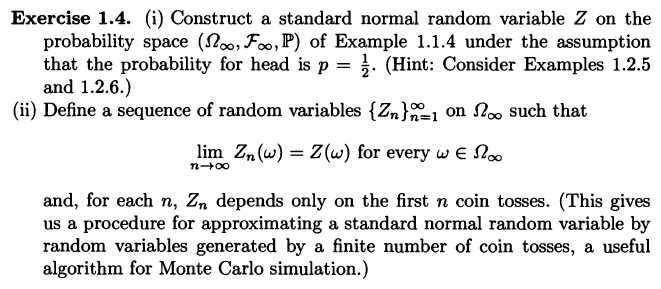
\includegraphics[width=14cm]{Exercise1p4.png}\\
	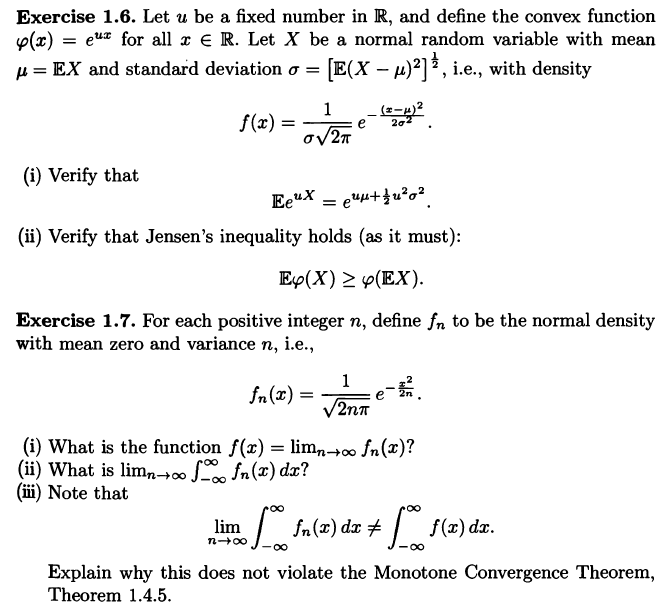
\includegraphics[width=14cm]{Exercise1p61p7.png}


%	\appendix
%%% \section{}
%%% \label{}
%
%%% References
%%%
%%% Following citation commands can be used in the body text:
%%% Usage of \cite is as follows:
%%%   \cite{key}         ==>>  [#]
%%%   \cite[chap. 2]{key} ==>> [#, chap. 2]
%%%
%
%%% References with bibTeX database:
%
%	\section{Reference}
	\bibliographystyle{elsarticle-harv}
	\bibliography{../MATH6740cit}
%
%%% Authors are advised to submit their bibtex database files. They are
%%% requested to list a bibtex style file in the manuscript if they do
%%% not want to use elsarticle-num.bst.
%
%%% References without bibTeX database:
%
%% \begin{thebibliography}{00}
%
%%% \bibitem must have the following form:
%%%   \bibitem{key}...
%%%
%
%% \bibitem{}
%
%% \end{thebibliography}

\end{document}



